\documentclass{standalone}
\usepackage{tikz}
\usetikzlibrary{arrows}
\begin{document}
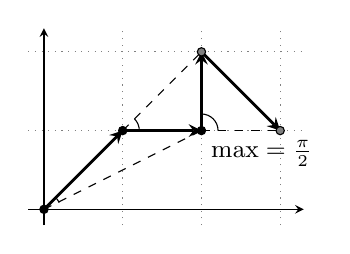
\begin{tikzpicture}[>=stealth]
\draw[step=1cm, color=gray, dotted] (-.2,-.2) grid (3.3,2.3);

\draw [->] (-.2,0) -- (3.3,0);
\draw [->] (0,-.2) -- (0,2.3);

\draw [line width=1pt, ->] (0,0)--(1,1);
\draw [line width=1pt, ->] (1,1)--(2,1);
\draw [line width=1pt, ->] (2,1)--(2,2);
\draw [line width=1pt, ->] (2,2)--(3,1);

\filldraw (0,0) circle (1.5pt)
          (1,1) circle (1.5pt)
		  (2,1) circle (1.5pt);
\filldraw[fill=gray]	  
          (2,2) circle (1.5pt)
	  	  (3,1) circle (1.5pt);
\draw[dashed] (0,0)--(2,1);
\draw[dashed] (1,1)--(2,2);
\draw[dashed] (2,1)--(3,1);

\draw([shift={(24:6pt)}]0,0) arc (24:45:6pt);		 
\draw([shift={(  0:6pt)}]1,1) arc (0:45:6pt);		 
\draw([shift={(  0:6pt)}]2,1) arc (0:90:6pt);		 
\draw (2,1) node[anchor=north west] {\small $\max = \frac{\pi}{2}$};
\end{tikzpicture}
\end{document}
